\documentclass[12pt,letterpaper]{report}
\usepackage[margin=0.75in]{geometry}
\usepackage[latin1]{inputenc}
\usepackage{amsmath}
\usepackage{amsfonts}
\usepackage{amssymb}
\usepackage{graphicx}
\usepackage{color}
\usepackage{fancyhdr}
\usepackage{minted}
\usepackage[T1]{fontenc}
\usepackage{inconsolata}
\usepackage{forest}
\usepackage{float}
\usepackage{pgfplots}
\usepackage{hyperref}
\pagestyle{fancy}
\fancyhead{}
\lhead{CS350}
\chead{Project Report}
\rhead{Caleb Boylan}
\author{Caleb Boylan}
\title{CS350 Project Report\\ Good Sorts and Multithreading\\ Fall 2018}
\date{}

\newcommand{\rust}[1]{\mintinline{rust}{#1}}

\begin{document}
\maketitle

	\section*{Project Description}

	For my project I decided I would implement some $\Omega(n^2)$ sorting algorithms: Bubble Sort, Insertion Sort, and Selection Sort as well as some $\Omega(nlog(n))$ algorithms: QuickSort and Merge Sort. My main feature for this project is multithreading QuickSort and Merge Sort and analyzing the performance benefits and draw backs, for this reason I won't focus much on the $\Omega(n^2)$ algorithms in my project report. All of my work was done using the Rust programming language, which aims to be a fast and memory safe language.\\
	
	All of my code used for this project is available on my github at:\\ \url{https://github.com/squidboylan/rust_sort}

	\section*{Implementation}
	
	\subsection*{Bubble Sort}
	
	Bubble Sort\cite{bubble_sort} is one of the easiest algorithms to implement. Bubble Sort is done by iterating through the whole array and swapping adjacent items if they are out of order. We do this until the whole array is sorted, then we stop when we iterate through the whole array without swapping any items as that means our array is sorted. My implementation can be seen in Figure 1.  One thing to note about my algorithm is it uses Rust's generics to allow sorting of any type that implements \rust{PartialOrd} which is what provides the comparison operators, which of course are essential to sorting. This includes all of Rust's primitive integer types, as well as the \rust{char} type which represents unicode code points. It will also work for user created types as long as they implement \rust{PartialOrd} for their type.
	
	\begin{figure}[H]
	\begin{minted}{rust}
pub fn bubble_sort<T: PartialOrd>(vals: &mut [T]) {
    if vals.len() == 0 {
        return;
    }
    let mut end = vals.len() - 1;
    loop {
        let mut swapped = false;
        let mut i = 0;
        while i < end {
            if vals[i] > vals[i+1] {
                vals.swap(i, i+1);
                swapped = true;
            }
            i += 1;
        }
        if !swapped {
            break;
        }
        end -= 1;
    }
}
    \end{minted}
    \caption{Bubble Sort}
\end{figure}

	\subsection*{Selection Sort}
	I decided to implement the iterative form of Selection Sort\cite{selection_sort} to prevent the performance costs of stack allocation and to prevent stack overflows with large array sizes. My implementation of Selection Sort is fairly basic, start from the next largest index and find the next largest value in the array, then put the next largest value in the array into the next largest index. Do this until the whole array is sorted. This could also be done in the opposite order, starting from index $0$ and finding the next smallest value in the array instead. Figure 2 shows my implementation of Selection Sort. Again I use Rust's generics to allow sorting of any type that implements \rust{PartialOrd}.

	\begin{figure}[H]
	\begin{minted}{rust}
pub fn selection_sort<T: PartialOrd>(vals: &mut [T]) {
    if vals.len() == 0 {
        return;
    }
    let mut curr = vals.len() - 1;
    while curr > 0 {
        let mut i = curr;
        let mut j = curr;
        while j > 0 {
            if vals[j-1] > vals[i] {
                i = j-1;
            }
            j -= 1;
        }
        vals.swap(i, curr);
        curr -= 1;
    }
}
	\end{minted}
	\caption{Selection Sort}
\end{figure}

	\subsection*{Insertion Sort}
	My implementation of insertion sort\cite{insertion_sort} is fairly simple as well. Start at index $1$ and insert it into the sorted sub array in it's correct location. Then continue to do the same for each larger index. We don't start at index $0$ as inserting index $0$ into an empty sorted sub array is the same as just starting with index $1$. My implementation can be seen in figure 3. Again I use generics so it can be run on any type that implements \rust{PartialOrd}.
	
	\begin{figure}[H]
	\begin{minted}{rust}
pub fn insertion_sort<T: PartialOrd>(vals: &mut [T]) {
    let mut i = 1;
    while i < vals.len() {
        let mut j = i;
        while j > 0 && vals[j] < vals[j-1] {
            vals.swap(j, j-1);
            j -= 1;
        }
        i += 1;
    }
}
	\end{minted}
	\caption{Insertion Sort}
\end{figure}
	
	\subsection*{Merge Sort}

	Merge sort\cite{merge_sort} is made up of two functions, one that splits the array into two equal sizes (or one that is 1 larger than the other), and a function that merges the two sorted arrays into one sorted large array. First I will talk about the splitting function \rust{merge_sort} shown in figure 4. First it splits the array into two pieces and clones them (Lines 3 - 9). Then it recursively calls itself on each sub array (Lines 10 and 11). Then once those calls return it calls the merge function which merges the two sorted sub arrays into the original array passed in as an argument. This is done for all arrays of $len > 1$. Note that our function only takes a $slice$ as an argument. This is because slices are just fat pointers to arrays, which means they contain the length of our array in them and we don't have to pass that manually. This implementation also uses approximately $n + n/2 + n/4 ... n/n = 2n$ extra memory.

	\begin{figure}[H]
    \begin{minted}[linenos]{rust}
pub fn merge_sort<T: PartialOrd + Clone>(vals: &mut [T]) {
    if vals.len() > 1 {
        let mut left;
        let mut right;
        {
            let tmp = vals.split_at(vals.len()/2);
            left = tmp.0.to_vec();
            right = tmp.1.to_vec();
        }
        merge_sort(&mut left);
        merge_sort(&mut right);
        merge(vals, &mut left, &mut right);
    }
}
    \end{minted}
    \caption{Merge Sort}
\end{figure}

	The implementation of the \rust{merge} function is fairly simple as well as shown in figure 5. We iterate through each array simultaneously and take the next smallest array from the next elements and put it in our $vals$ array. If we iterate through one array completely, we take any left over values from the other array and put them at the end of our $vals$ array.

	\begin{figure}[H]
    \begin{minted}[linenos]{rust}
pub fn merge<T: PartialOrd + Clone>(vals: &mut [T], left: &mut [T], right: &mut [T]) {
    let mut x = 0;
    let mut y = 0;
    let mut i = 0;
    while x < left.len() && y < right.len() {
        if left[x] <= right[y] {
            vals[i] = left[x].clone();
            x += 1;
            i += 1;
        } else if left[x] > right[y] {
            vals[i] = right[y].clone();
            y += 1;
            i += 1;
        }
    }
    while x < left.len() {
        vals[i] = left[x].clone();
        x += 1;
        i += 1;
    }
    while y < right.len() {
        vals[i] = right[y].clone();
        y += 1;
        i += 1;
    }
}
    \end{minted}
    \caption{Merge}
\end{figure}

	Both of our functions have a new generic type bound: \rust{Clone}. This signals to the Rust compiler that it is possible to clone data of our generic type \rust{T}. This is important because my implementation of mergesort clones the array into two smaller sub arrays and the compiler has to know this is possible.

	\subsection*{Multithreaded Merge Sort}
	
	This is one of the most interesting algorithms I implemented. Merge sort is a divide and conquer algorithm, which makes it easy to divide the work and give each half of the work to new threads to finish, then combine our results in the parent thread. This requires a new but similar implementation of the \rust{merge_sort} function but not the \rust{merge} function. The multithreaded \rust{merge_sort} function is shown in figure 6.
	
	First, our new function has a new bound for the generic type: \rust{Send}. This signals to the Rust compiler that it is safe to pass this data over thread boundaries, as not all data is. The good thing is that most types implement \rust{Send} so it doesn't restrict us much.
	
	Second, our new function takes an extra argument \rust{depth}, which signifies at which depth in the recursion to spawn the last threads. This spawns threads in a tree like manner, where the tree is complete and has a height of \rust{depth + 1} (because there is always the first thread that starts the program). The threads at each level are also merged by their parent threads. Doing it this way serves one main purpose: if we have a tree of threads and the tree is not complete, we will bottleneck ourselves because some threads will have more work than others. Figure 6 shows the tree of threads formed when \rust{depth = 2}.

	\begin{figure}[H]	
	\begin{center}
	\begin{forest}
	[T1
		[T2
			[T4]
			[T5]
		]
		[T3
			[T6]
			[T7]
		]
	]
	\end{forest}
    \caption{Multithreaded Merge Sort depth = 2}
    \end{center}
\end{figure}

	
	Finally, Lines 13 - 20 use the Rust crate \rust{crossbeam} to 2 spawn scoped threads, 1 for each sub array. This is important because threads in the Rust \rust{std} library are not scoped and cause lifetime issues as our threads could outlive the data they are working on! This is the exact problem Rust tries to solve so we have to use a special library to do the work for us and it ensures our threads don't outlive our data. This change also incurs extra memory costs because we are working in parallel, approximately $(depth + 1) * (n) + (n/2 + n/4 + ... n/n) = ((depth + 1) * n) + n = n(depth) + 2n$ extra memory is used. This means with more threads comes the cost of more memory, but the relation is logarithmic to the number of threads.
	
	\begin{figure}[H]
    \begin{minted}[linenos]{rust}
pub fn merge_sort_multithreaded<T: PartialOrd + Clone + Send>(vals: &mut [T], depth: usize) {
    if vals.len() == 1 {
        return;
    }
    let mut left;
    let mut right;
    {
        let tmp = vals.split_at(vals.len()/2);
        left = tmp.0.to_vec();
        right = tmp.1.to_vec();
    }
    if depth > 0 {
        crossbeam::scope(|scope| {
            scope.spawn(|| {
                merge_sort_multithreaded(&mut left, depth - 1);
            });
            scope.spawn(|| {
                merge_sort_multithreaded(&mut right, depth - 1);
            });
        });
    } else {
        merge_sort(&mut left);
        merge_sort(&mut right);
    }
    merge(vals, &mut left, &mut right);
}
    \end{minted}
    \caption{Merge Sort Multithreaded}
\end{figure}
	
	\subsection*{QuickSort}
	
	QuickSort\cite{quick_sort} uses partitioning to sort an array in $\Omega(nlog(n))$ time. It does this by running a partition function at every step, then recursively calling itself on the left and right side of the array that were split using partitioning.
	
	My partitioning function uses a basic Hoare partition algorithm. I chose Hoare for one main reason, it out performs Lomuto as it doesn't do as many unnecessary swaps. Hoare partitioning works by having two indices that start on each end of the array, then move them towards the middle until you find an element that belongs on the opposite side of the array. For the index on the left it means the current element is larger than or equal to the pivot, for the right it means the current element is smaller than the pivot. Then when each index has an element that needs to be swapped, you swap them. Finally when the indices cross or land on the same element, swap the pivot element, in our case 0, with the index from the right. Figure 8 shows my Hoare partitioning function.
	
	\begin{figure}[H]
    \begin{minted}{rust}
pub fn partition<T: PartialOrd>(vals: &mut [T]) -> usize {
    let mut i = 1;
    let mut j = vals.len() - 1;
    loop {
        while i < vals.len() && vals[i] < vals[0] {
            i += 1;
        }
        while vals[j] >= vals[0] {
            if j == 0 {
                break;
            }
            j -= 1;
        }
        if i >= j {
            break;
        }
        vals.swap(i, j);
        i += 1;
        j -= 1;
    }
    vals.swap(0, j);
    j
}
    \end{minted}
    \caption{Hoare Partition}
\end{figure}

	Figure 9 shows my \rust{quicksort} function. It is fairly simple, first we partition the array using the Hoare partition on line 4. Then on lines 5 - 7 we create two new subarrays, which are pointers to the existing array, but have lengths and starting points such that \rust{left} contains $[0, pivot)$ and \rust{right} contains $(pivot, len)$. Finally we recursively call our function on the left and right sub arrays.

	\begin{figure}[H]
    \begin{minted}[linenos]{rust}
pub fn quicksort<T: PartialOrd>(vals: &mut [T]) {
    if vals.len() > 1 {
        let pivot = partition(vals);
        // Split vals into two arrays, left contains [0, pivot), the contains (pivot, len)
        let tmp = vals.split_at_mut(pivot);
        let left = tmp.0;
        let right = tmp.1.split_at_mut(1).1;
        quicksort(left);
        quicksort(right);
    }
}
    \end{minted}
    \caption{Quick Sort}
\end{figure}
	
	\subsection*{Multithreaded QuickSort}
	
	A multithreaded quicksort function is made the same way as the multithreaded merge sort. First we partition the array using Hoare partitioning, then we call \rust{quicksort_mutlithreaded} on the subarrays in parallel using crossbeam if $depth > 0$. This forms the same tree of threads that the multithreaded merge sort did as seen in Figure 10.
	
\begin{figure}[H]	
	\begin{center}
	\begin{forest}
	[T1
		[T2
			[T4]
			[T5]
		]
		[T3
			[T6]
			[T7]
		]
	]
	\end{forest}
    \caption{Multithreaded QuickSort depth = 2}
    \end{center}
\end{figure}

	Our multithreaded QuickSort also requires our generic type \rust{T} implements \rust{Send}. This is for the same reason as described for Merge Sort, not all data is safe to pass across thread boundaries, this signals to the compiler that it is safe to pass our data of type \rust{T} across thread boundaries. Unlike the multithreaded Merge Sort implementation, multithreaded QuickSort doesn't use any extra memory (other than the size of the extra stacks for our new threads of course). Figure 11 contains my implementation of multithreaded QuickSort.
	
	\begin{figure}[H]
    \begin{minted}[linenos]{rust}
pub fn quicksort_multithreaded<T: PartialOrd + Send>(vals: &mut [T], depth: usize) {
    if vals.len() > 1 {
        let pivot = partition(vals);
        let tmp = vals.split_at_mut(pivot);
        let left = tmp.0;
        let right = tmp.1.split_at_mut(1).1;
        if depth > 1 {
            crossbeam::scope(|scope| {
                scope.spawn(|| {
                    quicksort_multithreaded(left, depth - 1);
                });
                scope.spawn(|| {
                    quicksort_multithreaded(right, depth - 1);
                });
            });
        } else {
            quicksort(left);
            quicksort(right);
        }
    }
}
    \end{minted}
    \caption{Multithreaded Quick Sort}
\end{figure}

\newpage

	\section*{Testing}
	
	Testing was done using the built in unit testing features in the Rust build manager $cargo$. I built a few helper functions that take a sorting algorithm as an argument:
	
	\begin{figure}[H]
	\begin{minted}{rust}
    fn test_function_rand(f: fn(&mut [u64])) {
        for i in 0..1024 {
            let mut numbers = rand_vec_u64(i);
            let mut sorted = numbers.clone();
            sorted.sort_unstable();
            f(numbers.as_mut_slice());
            assert_eq!(numbers, sorted);
        }
    }
 	\end{minted}
     \caption{Test sorting a random vector}
\end{figure}

	\begin{figure}[H]
	\begin{minted}{rust}
    fn test_function_sorted(f: fn(&mut [u64])) {
        for i in 0..1024 {
            let mut numbers = sorted_vec_u64(i);
            let mut sorted = numbers.clone();
            sorted.sort_unstable();
            f(numbers.as_mut_slice());
            assert_eq!(numbers, sorted);
        }
    }
 	\end{minted}
     \caption{Test sorting a sorted vector}
\end{figure}

	\begin{figure}[H]
	\begin{minted}{rust}
    fn test_function_reverse_sorted(f: fn(&mut [u64])) {ge
        for i in 0..1024 {
            let mut numbers = reverse_sorted_vec_u64(i);
            let mut sorted = numbers.clone();
            sorted.sort_unstable();
            f(numbers.as_mut_slice());
            assert_eq!(numbers, sorted);
        }
    }
 	\end{minted}
     \caption{Test sorting a reverse sorted vector}
\end{figure}

	I also implemented similar functions that accept multithreaded sorting function as an argument. I will not include these as they are the same as the single threaded functions but they also test with depth values of [0, 3).

	Then I built a wrapper for each sorting function that tests a known vector and uses the helper functions to test random, sorted, and reverse sorted vectors. This is the function that cargo builds and compiles as a unit test. The wrapper test function for insertion sort is shown in figure 15:

	\begin{figure}[H]
	\begin{minted}{rust}
    #[test]
    fn insertion_sort_test() {
        let mut vals = [1, 5, 4, 6, 7, 2, 3];
        insertion_sort(&mut vals);
        assert_eq!(vals, [1, 2, 3, 4, 5, 6, 7]);
        test_function_rand(insertion_sort);
        test_function_sorted(insertion_sort);
        test_function_reverse_sorted(insertion_sort);
    }
	\end{minted}
    \caption{Insertion Sort Test function}
\end{figure}

		
\newpage

	\section*{Benchmarks}
	
	All benchmarks were done using a \rust{Vec} of Rust's unsigned 64 bit integers, \rust{u64}, though my functions are all generic and should run similarly for the other data types that implement the necessary features to use my functions assuming the compare and clone operations have similar costs to \rust{u64}. \rust{Vec} was also chosen as they it is the defacto dynamically allocated array in Rust, but my functions would also work on statically allocated arrays as well. I used the Rust library $criterion$ for managing benchmarks. This made adding and collecting data much easier than doing it manually. The figure below shows an example benchmark function using criterion.

	\begin{figure}[H]
	\begin{minted}{rust}
fn merge_sort_10(c: &mut Criterion) {
    let arr_size = 10;
    c.bench_function("merge sort 1T 10", move |b| {
        b.iter_with_setup(
            || rand_vec_u64(arr_size), move |mut vals: Vec<u64>| merge_sort(&mut vals)
        );
    });
}
	\end{minted}
    \caption{Merge Sort n=10 benchmark}
\end{figure}


	This benchmark uses criterion to benchmark the \rust{merge_sort} function across many different random arrays generated with my \rust{rand_vec_u64} function (shown in figure 17). Criterion benchmarks this function a number of times based on how long it takes to run, this is so fast functions have more accurate benchmarks, and slow functions don't take forever to benchmark.
	
	\begin{figure}[H]
	\begin{minted}{rust}
pub fn rand_vec_u64(size: u64) -> Vec<u64> {
    let mut rng = rand::thread_rng();
    (0..size).map(|_| { rng.gen_range(0, size) }).collect()
}
	\end{minted}
    \caption{rand\_vec\_u64}
\end{figure}

	\rust{rand_vec_u64} looks intimidating, but all it does is generates a random number in the range of $[0..size)$, $size$ times and then puts them into a vector.

	\subsection*{Hardware}
	
	All benchmarks were run on my desktop, the specifications are as follows:\\
	
	CPU: AMD Ryzen 7 1700 8C/16T @3.0Ghz boost to 3.7Ghz\\
	
	L1: 32KB per core\\
	
	L2: 512KB per core\\
	
	L3: 8MB per core cluster (4 cores per cluster for 2 clusters per CPU)\\
	
	RAM: 16GB@2133Mhz DDR4\\
	
	OS: Ubuntu 18.04 with Linux 4.15.0-39\\
	
	Rustc: 1.30.1 \\
	
	This information will be key to analyzing the real world performance of my algorithms, particularly with the multithreaded algorithms and how they interact with the cache.
	
	\subsection*{$\Omega(n^2)$ Algorithms}
	
	Table 1 shows the average case performance of Bubble Sort, Insertion Sort, and Selection Sort. This is included only for completeness, but is not the main focus of my paper so I will not analyze the data in depth.
	
\begin{table}[h!]
  \begin{center}
    \caption{$n^2$ algorithms average case performance (ms)}
    \label{tab:table1}
    \begin{tabular}{l|r|r|r}
      \textbf{array size} & \textbf{Bubble Sort} & \textbf{Insertion Sort} & \textbf{Selection Sort}\\
      \hline
      10 & 0.00019165 & 0.00013784 & 0.00018429\\
      100 & 0.013159 & 0.0053858 & 0.0062227\\
      1000 & 0.9629 & 0.47548 & 0.33737\\
      10000 & 109.89 & 46.927 & 27.88\\
      100000 & 14518 & 4685.5 & 2717.2\\
    \end{tabular}
  \end{center}
\end{table}	

	\subsubsection{Analyzing the Data}

	The $\Omega(n^2)$ algorithms performed as expected. They perform well and all exhibit the theoretical $n^2$ asymptotic complexity. We also see that Selection Sort outperforms the others, this makes sense as Selection Sort does fewer swaps than the others. Another thing we see here is that for extremely small arrays, our $\Omega(n^2)$ algorithms outperform some of our $\Omega(nlog(n))$ algorithms (benchmarks shown in table 2 and table 3), this is because although they are $\Omega(n^2)$, their basic operations are much cheaper. This is because Merge Sort copies data and both Merge Sort and QuickSort are recursive, whereas our $\Omega(n^2)$ algorithms are all iterative.
	
	\subsection*{Merge Sort}
	
	Table 2 shows the average case performance of Merge Sort with 1, 2, 4, and 8 threads, across small to large array sizes. It also includes the Rust stable sort as a reference, though it is worth noting that the Rust stable sort is not Merge Sort, but rather an algorithm based on Tim Sort \cite{sort_stable}, which is why the performance is not identical.
	
	\begin{table}[H]
  \begin{center}
    \caption{Merge Sort average case performance (ms)}
    \label{tab:table1}
    \begin{tabular}{l|r|r|r|r|r}
      \textbf{array size} & \textbf{Merge Sort} & \textbf{Merge Sort 2T} & \textbf{Merge Sort 4T} & \textbf{Merge Sort 8T} & \textbf{Rust Stable}\\
      \hline
      10 & 0.00058715 & 0.094553 & 0.25464 & 0.47185 & 0.00011766\\
      100 & 0.0078244 & 0.12919 & 0.2813 & 0.50046 & 0.0026704\\
      1000 & 0.091386 & 0.23817 & 0.33548 & 0.54398 & 0.040033\\
      10000 & 1.0731 & 1.7214 & 1.2303 & 1.3732 & 00.54913\\
      100000 & 12.539 & 15.542 & 9.87 & 7.1333 & 6.7592\\
      1000000 & 145.78 & 90.667 & 69.615 & 54.31 & 83.79\\
    \end{tabular}
  \end{center}
\end{table}

 	The graph below shows the average case performance of Merge Sort on arrays of size 1m - 20m.

\begin{center}
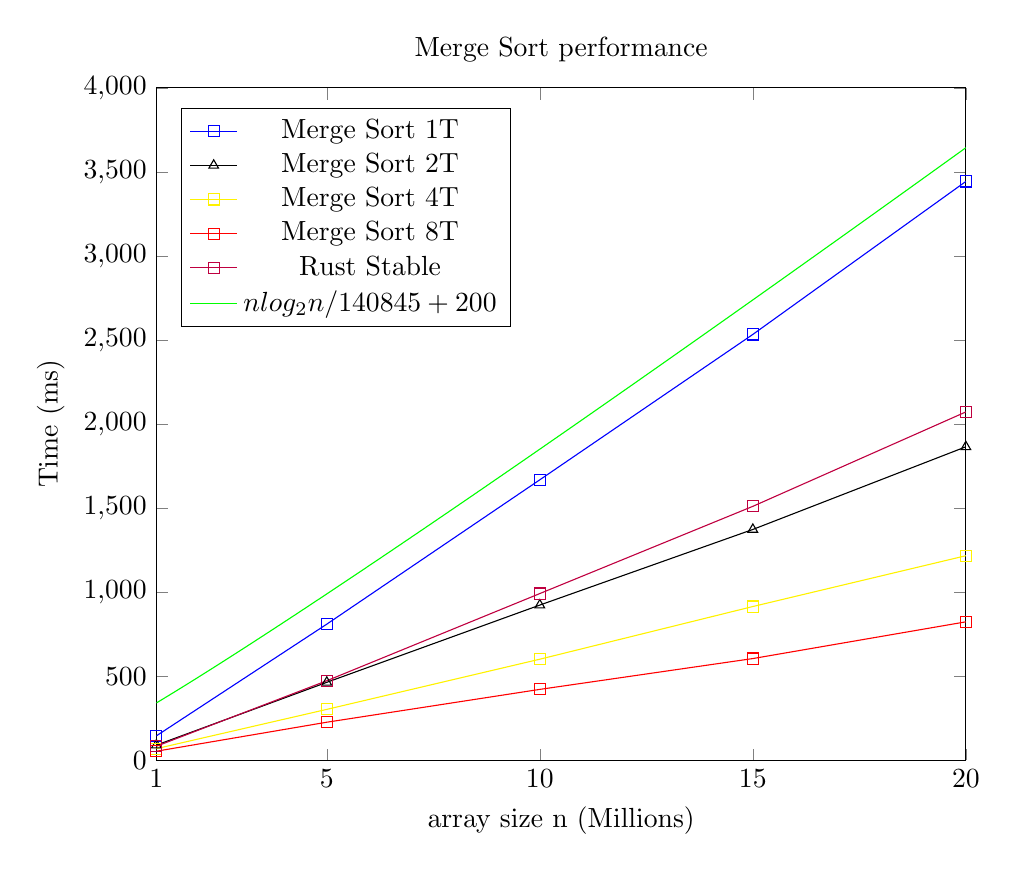
\begin{tikzpicture}
\begin{axis}[
    title={Merge Sort performance},
    xlabel={array size n (Millions)},
    ylabel={Time (ms)},
    xmin=1, xmax=20,
    ymin=0, ymax=4000,
    xtick={1, 5, 10, 15, 20},
    ytick={0,500,1000,1500,2000,2500,3000,3500,4000},
    grid style=dashed,
    legend pos=north west,
    scale=1.5,
]
 
\addplot[
    color=blue,
    mark=square,
    ]
    coordinates {
    (1,145.78)(5,810.18)(10,1668.8)(15,2533.5)(20,3443.3)
    };
    \addlegendentry{Merge Sort 1T}
    
\addplot[
    color=black,
    mark=triangle,
    ]
    coordinates {
    (1,90.667)(5,464.1)(10,923.63)(15,1373.4)(20,1865.1)
    };
    \addlegendentry{Merge Sort 2T}
    
\addplot[
    color=yellow,
    mark=square,
    ]
    coordinates {
    (1,69.615)(5,303.23)(10,601.68)(15,914.99)(20,1217.2)
    };
    \addlegendentry{Merge Sort 4T}

\addplot[
    color=red,
    mark=square,
    ]
    coordinates {
    (1,54.31)(5,226.86)(10,422.13)(15,605.48)(20,823.91)
    };
    \addlegendentry{Merge Sort 8T}
    
\addplot[
    color=purple,
    mark=square,
    ]
    coordinates {
    (1,83.79)(5,473.58)(10,992.13)(15,1510.9)(20,2072.4)
    };
    \addlegendentry{Rust Stable}


    
\addplot [
    domain=1:20 ,
    samples=100, 
    color=green,
]{1000000 * x * log2(x * 1000000) * .0000071 + 200};
\addlegendentry{$nlog_{2}n/140845 + 200$}

\end{axis}
\end{tikzpicture}
\end{center}

	\subsubsection{Analyzing the Data}
	
	I will only analyze Merge sort average case performance as it has the same complexity as its best and worst case performance. Merge Sort performs fairly well and has $\Omega(nlog(n))$ complexity for all cases. This is exhibited in our benchmarks in Table 2.
	
	The most interesting part of this project is how Merge Sort benefits from multithreading. With small arrays, single threaded merge sort out performs the multithreaded version. With large arrays, the multithreaded versions beat the single threaded version, but they are not \textbf{number of threads} times faster, which is the theoretical ideal performance. This is likely the case for a few reasons. First, threads have a cost associated with them. Spawning a thread requires making a system call to the operating system, in this case Linux, which is a rather slow operation.
	
	Secondly, modern hardware tries to achieve high single core performance while also having good multicore performance. This is done by have a boost clock where when only 1 core is active, that core is boosted past the normal clock speed, in this case the clock is raised from 3.0Ghz, to 3.7Ghz, an approximately 23\% gain. This means when we have more cores, we don't get 2 cores running at the same high speed, but 2 cores running at a lower clock speed.
	
	It is also worth considering the effect of caching in our function. Memory operations are slow because RAM hardware is much slower than CPU memory (registers). Hardware designers try to alleviate this by adding small, but quick memory between the CPU and our RAM called caches. There are 3 caches on my hardware L1, L2, and L3, L1 being the smallest and fastest and L3 being the largest and slowest.
	
	When we add threads to our algorithm, they run on different cores, which do not share L1 and L2 caches, meaning the new thread must retrieve the memory from the L3 cache when it may have already been in the L1 cache of the parent thread. You might also wonder why we have diminishing returns for more threads. First of all not all of the workload can be spread across our cores, the merging of each 2 child threads is done by the parent, meaning at the end of our algorithm, we sort $n$ items on a single thread. Next, on my hardware with 8 physical cores, there are 2 L3 caches, shared by clusters of 4 cores. This means that when we have 4 threads, they share an L3 cache, but when we have 8 threads, not all of the threads share an L3 cache, which will cause memory operations to be slower and have more cache misses as memory will have to be passed between the two L3 caches. This is also why we see better performance with 8 threads when our data usage is more than 8MB (the size of each L3 cache), because we cant fit everything into the L3 cache anyways, so having more threads that have a separate L3 cache has a smaller negative effect. For this reason I think the performance would quite a bit better if we had 1 large 16MB L3 cache shared between all 8 cores.
	
	Altogether this means the sweet spot for multithreading is where the cost of spawning threads, cache misses, and lower multicore clock speeds is outweighed by the amount of time saved by doing work in parallel. This of course depends on the hardware and array size.
	
	It is also worth noting that although my single threaded Merge Sort implementation does not outperform the built in Rust stable sort for small arrays, it outperforms it with large arrays and multiple numbers of threads. This is great, though it does not mean that my function is better as the Rust built in sort does more work with less CPU power, meaning it uses less power to do the same amount of work, even if it is a bit slower.
	
	\subsection*{QuickSort}
	
	Table 3 contains the average case performance of QuickSort with 1, 2, 4, and 8 threads across small to large arrays. It also contains the Rust unstable sorting function as reference, but this algorithm is not pure QuickSort, it is a mix of Heap Sort and QuickSort in order to boost performance \cite{sort_unstable}.
	
\begin{table}[H]
  \begin{center}
    \caption{QuickSort average case performance (ms)}
    \label{tab:table1}
    \begin{tabular}{l|r|r|r|r|r}
      \textbf{array size} & \textbf{QuickSort} & \textbf{QuickSort 2T} & \textbf{QuickSort 4T} & \textbf{QuickSort 8T} & \textbf{Rust Unstable}\\
      \hline
      10 & 0.00017656 & 0.00018011 & 0.083335 & 0.23617 & 0.0001153\\
      100 & 0.0028162 & 0.0029189 & 0.09326 & 0.24755 & 0.0015859\\
      1000 & 0.039267 & 0.041073 & 0.16769 & 0.28329 & 0.019437\\
      10000 & 0.50801 & 0.53123 & 1.1529 & 1.1414 & 0.24113\\
      100000 & 6.2214 & 6.5363 & 11.455 & 9.4812 & 2.7602\\
      1000000 & 73.097 & 76.802 & 68.875 & 61.5 & 41.307\\
    \end{tabular}
  \end{center}
\end{table}	

	The graph below shows the average case performance of Quick Sort on arrays of size 1m - 20m.

\begin{center}
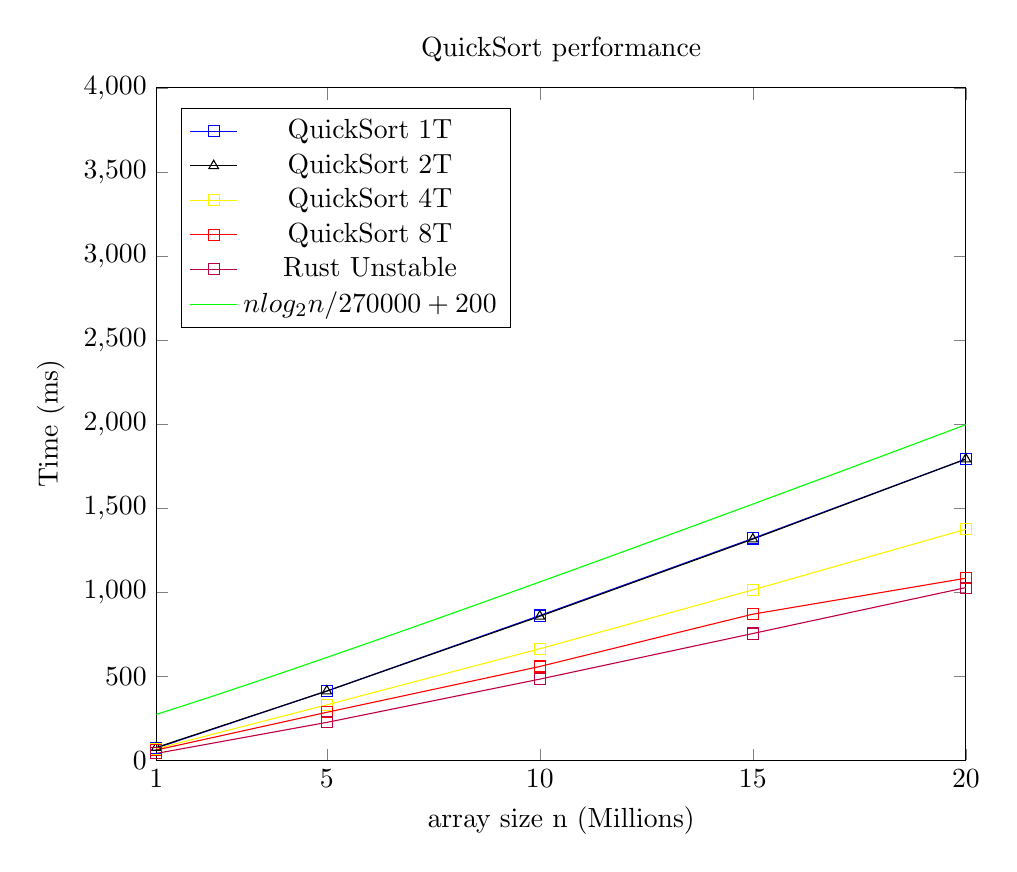
\begin{tikzpicture}
\begin{axis}[
    title={QuickSort performance},
    xlabel={array size n (Millions)},
    ylabel={Time (ms)},
    xmin=1, xmax=20,
    ymin=0, ymax=4000,
    xtick={1, 5, 10, 15, 20},
    ytick={0,500,1000,1500,2000,2500,3000,3500,4000},
    grid style=dashed,
    legend pos=north west,
    scale=1.5
]
 
\addplot[
    color=blue,
    mark=square,
    ]
    coordinates {
    (1,73.097)(5,412.44)(10,861.2)(15,1320)(20,1792.2)
    };
    \addlegendentry{QuickSort 1T}
    
\addplot[
    color=black,
    mark=triangle,
    ]
    coordinates {
    (1,76.802)(5,412.08)(10,856.79)(15,1315.9)(20,1792)
    };
    \addlegendentry{QuickSort 2T}
    
\addplot[
    color=yellow,
    mark=square,
    ]
    coordinates {
    (1,68.875)(5,330.19)(10,663.78)(15,1014)(20,1374.5)
    };
    \addlegendentry{QuickSort 4T}

\addplot[
    color=red,
    mark=square,
    ]
    coordinates {
    (1,61.5)(5,285.8)(10,558.3)(15,869.58)(20,1083.4)
    };
    \addlegendentry{QuickSort 8T}
    
\addplot[
    color=purple,
    mark=square,
    ]
    coordinates {
    (1,41.307)(5,225.74)(10,483.13)(15,754.42)(20,1027.5)
    };
    \addlegendentry{Rust Unstable}

    
\addplot [
    domain=1:20 ,
    samples=100, 
    color=green,
]{1000000 * x * log2(x * 1000000)/270000 + 200};
\addlegendentry{$nlog_{2}n/270000 + 200$}

\end{axis}
\end{tikzpicture}
\end{center}	
	
	\subsubsection{Analyzing the Data}

	I will not cover the QuickSort best case performance as it has the same complexity as the average case: $\Omega(nlog(n))$. I also will not cover the worst case performance as there are optimized versions that achieve $\Omega(nlog(n))$ complexity in worst case, unlike my naive version that is $\Omega(n^2)$ in the worst case.
	
	QuickSort performs extremely well, better than merge sort in the average case. QuickSort also fails to benefit from multithreading as much as Merge Sort does, this makes sense as it relies on the first \rust{depth} splits being best case, if they are not, we will have an uneven split of our workload between our threads. The benefit of QuickSort is that it uses less memory and doesn't require our type implements \rust{Clone}.
	
	We might be able to get better performance from multithreaded QuickSort by choosing a random pivot, and only spawning extra threads to do the work if our array is bigger than some size $m$, and the pivot is somewhere close to $m/2$. This would prevent us spawning threads to do little to no work when we get a bad pivot and would prevent spawning threads when the extra work is too small to benefit from. With optimization and large enough arrays I think QuickSort would be able to benefit from multithreading in similar ways to Merge Sort. If it does it would be much better than Merge Sort for unstable sorting as it doesn't require all the extra RAM, which could be limiting with Merge Sort and extremely large (1B+) arrays.
			
	\section*{Conclusion}
	
	While QuickSort is faster than Merge Sort, it benefits from multithreading. Merge Sort is able to be multithreaded easily for quite a bit more performance depending on array size and hardware. It would be possible to make a multithreaded Merge Sort that only spawns threads when $n > k$ where $n$ is the size of the array and $k$ is the size of array where multithreading provides a performance boost. This would provide good performance with small array sizes, while also achieving good performance with large array sizes. Though QuickSort should not be written off as it achieves more performance with less CPU time and it doesn't require extra ram, meaning for power sensitive and memory limited environments it is still the winner, such as mobile devices. It may also be possible to tune a multithreaded QuickSort function so that it performs better than multithreaded Merge Sort.

\begin{thebibliography}{9}

\bibitem{bubble_sort} 
Geeks for Geeks Bubble Sort,
\\\texttt{https://www.geeksforgeeks.org/bubble-sort/}

\bibitem{selection_sort} 
Geeks for Geeks Selection Sort,
\\\texttt{https://www.geeksforgeeks.org/selection-sort/}

\bibitem{insertion_sort} 
Geeks for Geeks Insertion Sort,
\\\texttt{https://www.geeksforgeeks.org/insertion-sort/}

\bibitem{merge_sort} 
Geeks for Geeks Merge Sort,
\\\texttt{https://www.geeksforgeeks.org/merge-sort/}

\bibitem{quick_sort} 
Geeks for Geeks Quick Sort,
\\\texttt{https://www.geeksforgeeks.org/quick-sort/}
 
\bibitem{sort_stable} 
Rust std stable sort source code,
\\\texttt{https://doc.rust-lang.org/src/alloc/slice.rs.html\#176}

\bibitem{sort_unstable} 
Rust std unstable sort source code,
\\\texttt{https://doc.rust-lang.org/src/core/slice/mod.rs.html\#1301}



\end{thebibliography}

\end{document}
